\section{Action--angle coordinates}\label{sec:aa}

\subsection{General approach}\label{sec:aa-general}

The action--angle module is where \galpy's numerical methods are
concentrated: root finding for the turning points of an orbit,
quadrature of the action integrals between them, and, for the
approximate methods, auxiliary orbit integrations. All of
\texttt{galpy.actionAngle} runs on the backends except for the interface
to the external torus-mapping code, which is excluded for good. The
public interface is unchanged: an \texttt{actionAngle} instance is set up
for a potential and called with phase-space positions, through
\texttt{\_\_call\_\_} for the actions, \texttt{actionsFreqs} for actions
and frequencies, and \texttt{actionsFreqsAngles} for all three; a call
with backend arrays, or with a potential that carries a backend
parameter, computes with that backend. Because these methods take a
variable number of positional arguments, they resolve the namespace and
promote scalars internally rather than through the coercion decorator
of the potentials. Derivatives are available with respect to the
phase-space position and, through the Python implementations, with
respect to the parameters of the potential; these parameter derivatives
agree with finite differences in which the potential and the
\texttt{actionAngle} instance are rebuilt from the perturbed parameter
to a few parts in $10^{10}$ for the St\"{a}ckel, adiabatic, and
spherical methods. \figurename~\ref{fig:aasens} shows the two kinds of
derivative for the isochrone potential, where the actions are known in
closed form: the derivatives of the radial and vertical actions with
respect to the radial velocity, and the derivative of the radial action
with respect to the scale radius of the potential, which is the
derivative that an inference loop uses when it adjusts the potential
to match measured actions.

\begin{figure*}[t!]
  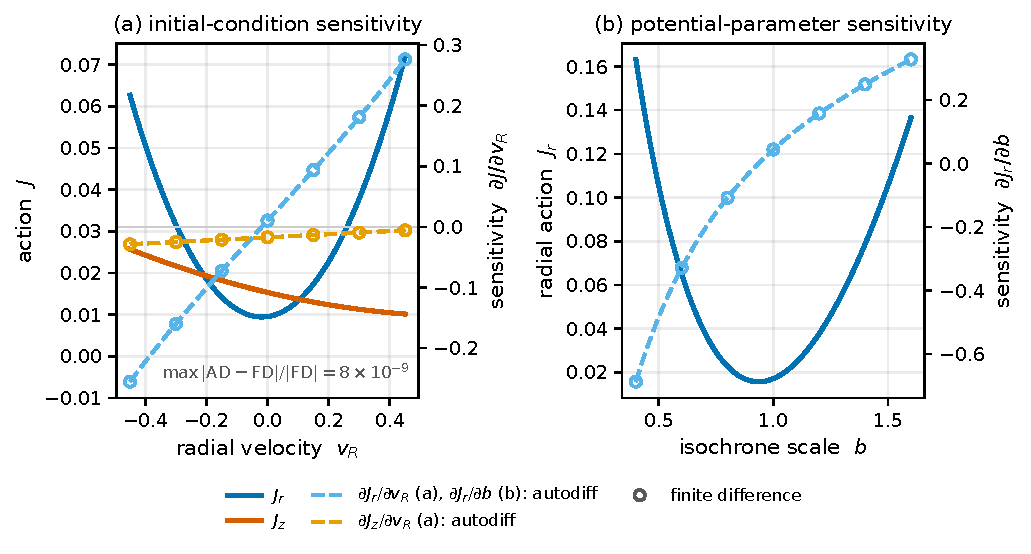
\includegraphics[width=\textwidth,clip=]{../figures/g18_actionangle_sensitivity/g18_actionangle_sensitivity.pdf}
  \caption{Derivatives of actions in the isochrone potential. Left: the
    radial and vertical actions of an orbit as a function of its radial
    velocity (solid, left axis) and their derivatives with respect to
    the radial velocity by automatic differentiation (dashed, right
    axis) with finite differences (circles). Right: the radial action as
    a function of the scale radius $b$ of the potential and its
    derivative with respect to $b$.}\label{fig:aasens}
\end{figure*}

\subsection{The St\"{a}ckel and adiabatic approximations}\label{sec:aa-staeckel}

\texttt{actionAngleStaeckel}, the workhorse for axisymmetric potentials,
has two implementations that behave differently under a backend. The
pure-\python\ path (\texttt{c=False}) was rewritten as part of this work
to be vectorized over phase-space points, where it previously looped
over them, and the same code runs under \numpy, \jax, and \torch: the
turning points are found by the fixed-count bisection and Newton
polish of \sectionname~\ref{sec:design-numerics}, and the action,
frequency, and angle integrals are evaluated with the same Gauss--Legendre
rule, in an anomaly variable that removes the square-root singularities
at the turning points, that the \cc\ implementation uses, such that the
two agree to machine precision. Everything on this path is
differentiable with respect to the phase-space coordinates and the
potential's parameters,
\begin{code}
def jr_of_a(a):
    aAS= actionAngleStaeckel(pot=MiyamotoNagaiPotential(a=a,b=0.3),
                             delta=0.4,c=False)
    return aAS(R,vR,vT,z,vz)[0].sum()
djr_da= jax.grad(jr_of_a)(0.5)
\end{code}
with the restriction that the derivative of the action integral is of
first order only. \figurename~\ref{fig:staeckelq} shows such a
derivative, of the radial and vertical actions of a Sun-like orbit with
respect to the flattening of a logarithmic halo, with the potential and
the St\"{a}ckel transformation rebuilt from $q$ inside the differentiated
function: the automatic derivative agrees with finite differences to
$10^{-10}$, at the bottom of the finite-difference error curve, and once
compiled it costs about a millisecond.

\begin{figure*}[t!]
  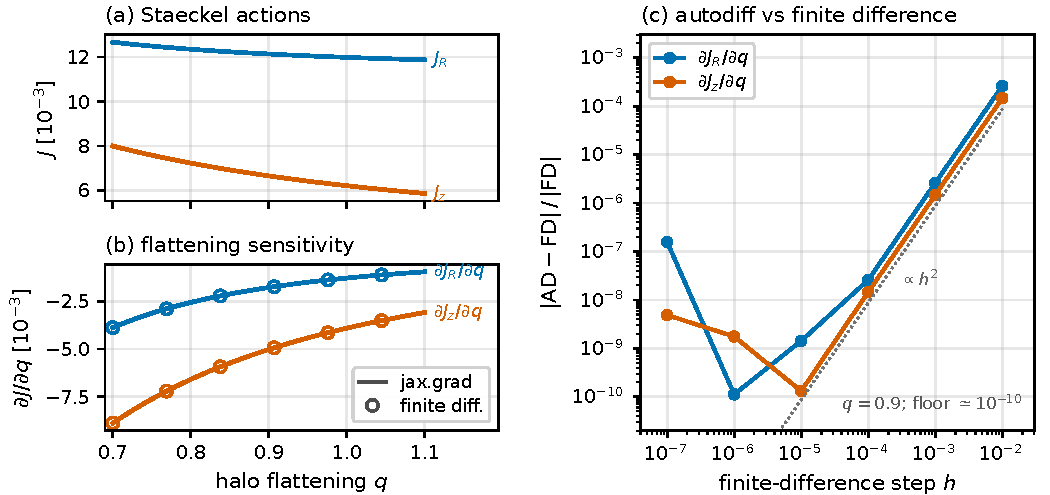
\includegraphics[width=\textwidth,clip=]{../figures/gA1_staeckel_param_sensitivity/gA1_staeckel_param_sensitivity.pdf}
  \caption{Derivatives of St\"{a}ckel actions with respect to a parameter
    of the potential. (a) The radial and vertical actions of a Sun-like
    orbit in a logarithmic halo as a function of its flattening $q$,
    computed with \texttt{actionAngleStaeckel(c=False)} at fixed focal
    length. (b) Their derivatives with respect to $q$ by \texttt{jax.grad}
    (lines) and by central finite differences in which the potential and
    the action--angle object are rebuilt (circles). (c) The relative
    difference between the two at $q=0.9$ as a function of the
    finite-difference step: the finite difference converges as $h^2$ onto
    the automatic derivative until rounding error takes over below
    $10^{-10}$.}\label{fig:staeckelq}
\end{figure*} The \cc\ path (\texttt{c=True}) is much faster for
small numbers of points and, on a backend, does more than before: the
\cc\ code computes, along with the actions, frequencies, and angles,
their Jacobian with respect to the five phase-space coordinates, and
this Jacobian is attached to the result as a custom derivative rule,
such that \texttt{jax.grad} or \torch's \texttt{backward} through a
\texttt{c=True} call costs one \cc\ call and a matrix product,
\begin{code}
aAS= actionAngleStaeckel(pot=MWPotential2014,delta=0.45,c=True)
def total_jr(R):
    return aAS(R,vR,vT,z,vz)[0].sum()
djr_dR= jax.jit(jax.grad(total_jr))(jnp.asarray([1.1,0.9]))
\end{code}
As for the orbit integrators, the \cc\ path gives derivatives with
respect to the phase-space position only, to first order, and the focal
length \texttt{delta} is a fixed number; derivatives with respect to the
potential's parameters require \texttt{c=False}. The estimate of the
focal length from the potential, \texttt{estimateDeltaStaeckel}, runs on
the backends and traces, such that a focal length estimated along an
integrated orbit can be part of a compiled program,
\begin{code}
delta= estimateDeltaStaeckel(MWPotential2014,o.R(ts),o.z(ts))
aAS= actionAngleStaeckel(pot=MWPotential2014,delta=delta,c=False)
jr,lz,jz= aAS(o.R(ts),o.vR(ts),o.vT(ts),o.z(ts),o.vz(ts))
\end{code}
The grid-based interpolated version,
\texttt{actionAngleStaeckelGrid}, builds its grid on the backend, such
that the grid lives on the GPU when the potential does and the
interpolated actions are differentiable with respect to the query
point; when the potential carries a parameter that is being
differentiated, the grid class delegates to the exact method, with a
warning, because the grid cannot be differentiated through its
construction. The adiabatic approximation follows the same pattern,
with a fused Jacobian in \cc\ for \texttt{c=True} and, for
\texttt{c=False}, the migrated spherical and vertical machinery for
its radial and vertical parts.

\subsection{Spherical potentials, the isochrone approximation, and the inverse transformation}\label{sec:aa-other}

The isochrone and harmonic-oscillator actions are closed forms and were
migrated by swapping the namespace. \texttt{actionAngleSpherical}
replaces its \scipy\ root finds and adaptive quadratures with the
shared root finder and a fixed-order Gauss--Legendre rule, with special
handling of circular and near-circular orbits, where the radial
integral degenerates, and of orbits that are unbound. The
\texttt{actionAngleIsochroneApprox} method of \citet{Bovy2014}
integrates an auxiliary orbit, and does so with the in-backend solvers
of \sectionname~\ref{sec:orbit-paths}; it is therefore differentiable
with respect to the potential's parameters, twice so under \jax\ with
the direct adjoint, and runs on a GPU.

The inverse transformation, from actions and angles to positions and
velocities, exists in \galpy\ for the isochrone and harmonic potentials
in closed form and for general one-dimensional potentials through
\texttt{actionAngleVerticalInverse}, which constructs a torus map by a
momentum-matched canonical transformation and tabulates it as a
function of the action. The construction---a root find for the maximum
excursion, a spectral sweep over the angle, a batched Gauss--Newton
solve for the anomaly, and Hermite-spline tables---and the evaluation
run natively on the backends, trace under compilation, and are
differentiable with respect to the action, the angle, and the
parameters of the potential, such that the family of tori can be
differentiated with respect to the parameters of the disk that
generates them. \figurename~\ref{fig:vinverse} demonstrates this for a
self-gravitating isothermal disk: the derivative of the tori with
respect to the velocity dispersion of the disk predicts the tori of a
nearby disk, agrees with finite differences to $10^{-10}$, and serves
as the Jacobian of a Levenberg--Marquardt fit of the disk's parameters to
stars scattered around three tori. In code, the tori of a family of disks
parametrized by their velocity dispersion are differentiated as
\begin{code}
def torus(sigma):
    disk= IsothermalDiskPotential(amp=1.,sigma=sigma)
    aAVI= actionAngleVerticalInverse(pot=disk,Es=Es,nta=128,
                                      setup_interp=True)
    return aAVI.xvFreqs(J,angles)[:2]  # (z, v_z) on the torus
z,vz= torus(0.5)
dz_dsigma,dvz_dsigma= jax.jacfwd(torus)(0.5)
\end{code}
The older construction modes of the
class, which use point transformations, are evaluated natively but
built on \numpy, and therefore cannot take a potential with backend
parameters.

\begin{figure*}[t!]
  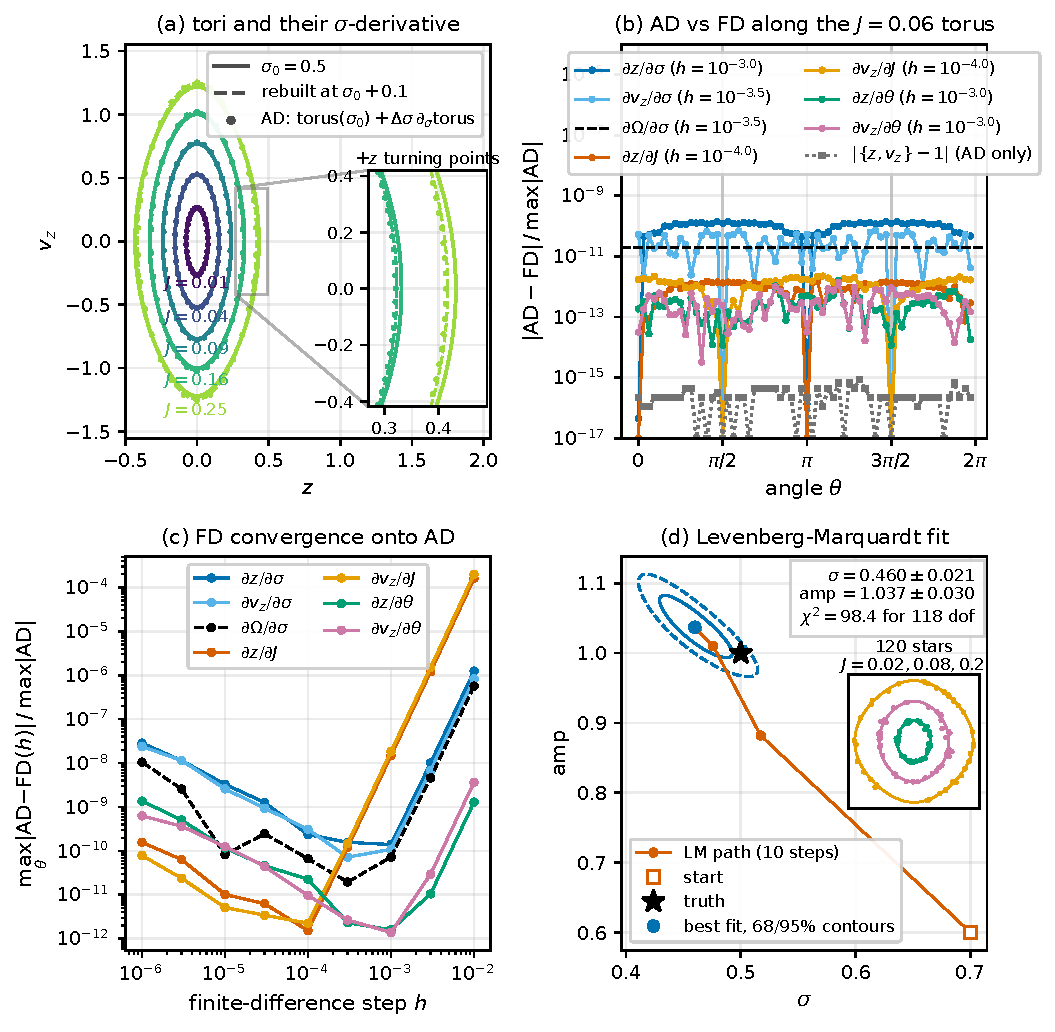
\includegraphics[width=\textwidth,clip=]{../figures/gV1_vertical_inverse/gV1_vertical_inverse.pdf}
  \caption{Differentiable inverse action--angle transformation in a
    self-gravitating isothermal disk with \texttt{actionAngleVerticalInverse}.
    (a) Tori at fixed actions for a disk with velocity dispersion
    $\sigma_0$ (solid), the same tori for a disk rebuilt with
    $\sigma_0+0.1$ (dashed), and the first-order prediction from the
    derivative of the tori with respect to $\sigma$ by automatic
    differentiation (points). (b) The difference between the derivatives
    of $z$, $v_z$, and the frequency with respect to $\sigma$, $J$, and
    $\theta$ along the $J=0.06$ torus and five-point finite differences,
    relative to the largest derivative. (c) The finite differences
    converge onto the automatic derivatives as $h^4$ until their
    round-off floor. (d) A Levenberg--Marquardt fit of $(\sigma,\,\mathrm{amp})$
    and 120 angles to 120 stars with noisy $(z,v_z)$ on three tori, using
    the automatic Jacobian; the fit converges in ten steps and the truth
    lies inside the 68\,\% contour.}\label{fig:vinverse}
\end{figure*}

\subsection{Speed}\label{sec:aa-speed}

Two things changed in the speed of the action--angle calculations. The
vectorized \python\ St\"{a}ckel path is now as fast as the single-threaded
\cc\ path for large numbers of points on the CPU, where the old
per-object loop was more than an order of magnitude slower, and this
holds for plain \numpy. And on a GPU, the same path under \torch\ or
compiled \jax\ overtakes the \cc\ path by an order of magnitude at
$10^5$ points, after a launch-bound floor of about a second; eager
\jax, which dispatches hundreds of small operations per call, is bound
by that dispatch and stays at a floor of several seconds. %TODO: Staeckel speed figure (g17) and its numbers after the re-measurement

The one-dimensional inverse transformation is shown in
\figurename~\ref{fig:vinvspeed}. Evaluating the torus map at $N$ angles
is fastest with \numpy\ for up to a few thousand angles, where the
backends pay their per-call overhead; compiled \jax\ overtakes it near
$N=10^4$ %TODO: 1-core jax CPU re-measurement (the current jax CPU series used up to 72 threads)
and on the H100 the same evaluation takes 11\,ms. The
backends find the angle with the same safeguarded Newton iteration as
\numpy, started at the requested angle. Constructing the map for a
family of $n_E$ energies is faster on every backend than on \numpy, by
an order of magnitude at $n_E=256$, because the batched Gauss--Newton
solve replaces a loop over tori; on a GPU the compiled construction takes
a few milliseconds whatever the size of the family. These numbers are for
the development machine and the H100 and should be read as orders of
magnitude.

\begin{figure*}[t!]
  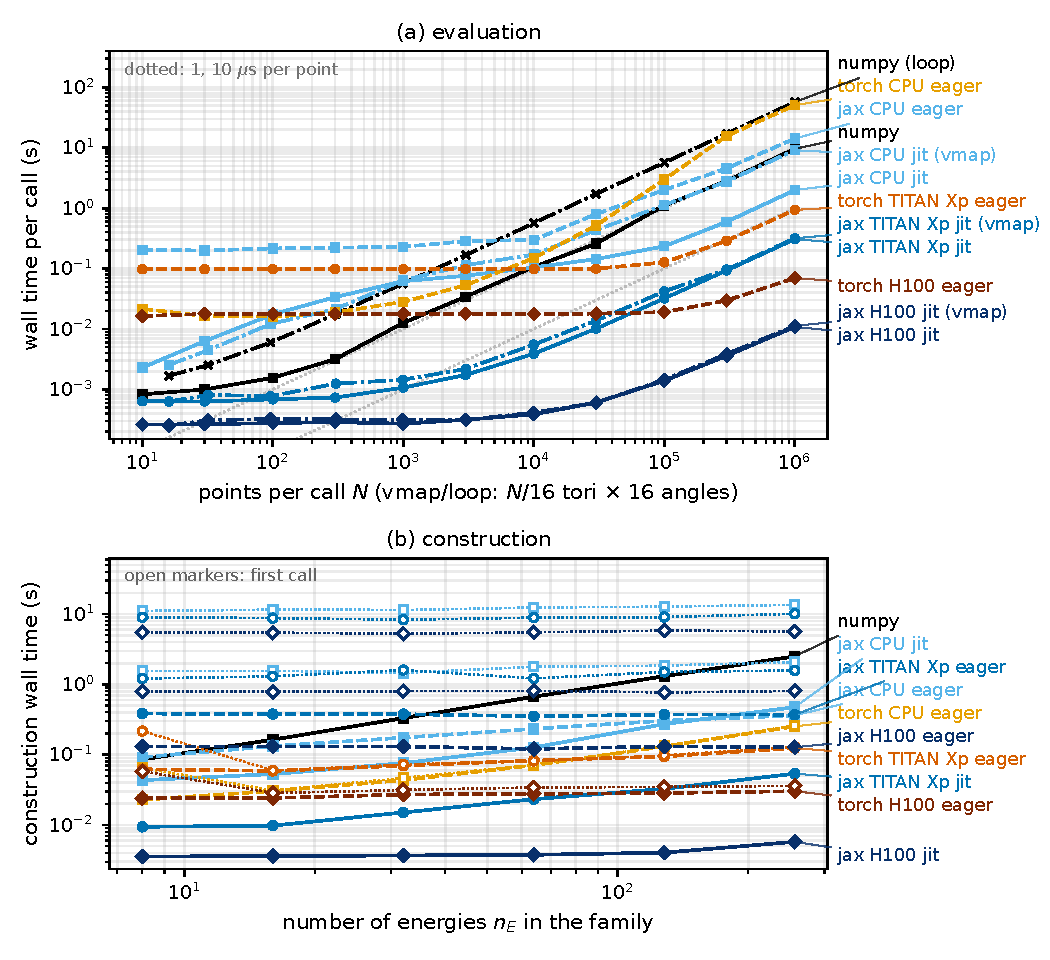
\includegraphics[width=\textwidth,clip=]{../figures/gV2_vertical_inverse_speed/gV2_vertical_inverse_speed.pdf}
  \caption{Speed of the one-dimensional inverse action--angle
    transformation, \texttt{actionAngleVerticalInverse}, for an
    isothermal disk. (a) Wall time to evaluate positions, velocities, and
    frequencies at $N$ angles on one torus (or, dash-dotted, at 16 angles
    on each of $N/16$ tori) with \numpy\ and on the backends on a single
    CPU core, the TITAN~Xp, and the H100; compilation time is excluded.
    (b) Time to construct the map for a family of $n_E$ energies, warm
    (filled markers) and on the first call (open markers), which for
    eager \jax\ includes compiling every operation for the new
    shapes.}\label{fig:vinvspeed}
\end{figure*}
